\documentclass[12pt,fleqn]{article}\usepackage{../common}
\begin{document}
Degisimsel Calculus (Calculus of Variations) ve Euler-Lagrange Denklemi

Degisimsel, Varyasyonel Calculus bir fonksiyon\textbf{el}in (dikkat
``fonksiyon'' degil) ekstrema (minimum / maksimum) ya da duragan
(stationary) oldugu noktalarin bulunmasi icin kullanilir.

Bir {\em fonksiyonel} bir veya daha fazla fonksiyonun
birlesimidir. Fonksiyonel girdi olarak bir fonksiyon alip sonuc olarak
bir sayisal deger hesaplayan bir ikinci fonksiyondur aslinda. Diger
bir tanim fonksiyonelin belli fonksiyon ``tipleri'', ``siniflari''
icin bir sayisal deger atamasi yaptigidir.

Degimsel calculus'un en temel, bilinen, standart problemi, sabit $x$
degerleri icin alttaki fonksiyonelin (entegralin) duragan oldugu
$\phi(x)$ fonksiyonlarini bulmaktir. Yine dikkat: Bulmaya calistigimiz
bir skalar $x$ degeri degil, bir veya daha fazla fonksiyondur.

\[ I(\phi)=\int_a^b F(x,\phi,\phi_x)dx \]

$\delta$ isareti varyasyon operatorudur, ve diferansiyel operatoru
$d$'ye oldukca benzer. $\phi(x)$'nin varyasyon operatoru uygulanmis
hali olan $\delta \phi(x)$'in tanimi, sabit bir $x$ degeri icin
herhangi (arbitrary), sonsuz ufaklikta (infinitesimal) bir degisim
demektir. Dogal olarak $x$'in sabit olmasi $\delta x = 0$ anlamina
gelir (bu esitligi birazdan formulumuzun aciliminda basitlestirme
amaci ile kullanacagiz). Fonksiyonelin duraganligi da $\delta I = 0$
demektir.

Degisimsel Calculus ve Euler-Lagrange aciliminin puf noktasi altta
birazdan gorecegimiz cebirsel islemlerle, $\delta \phi$'yi formulde
tek basina birakarak bir anlamda duraganlik mantiginin disina
atmasidir. Oyle bir $\phi(x)$ buluyoruz ki ondan $\delta$ sapmalari
var, ama biz oraya degil, formulun geri kalanina bakiyoruz, formulun o
tarafinda ustunde sapmalar olmayan $\phi$ ile islemler yapacagiz, ve
optimal bir $\phi$ fonksiyonu bulacagiz.

$I$ fonksiyoneli pek cok fizik, diger tur problemlerde ortaya cikan
bir formdur. Minimize edilmeye ugrasilan bir fonksiyonel var ise,
degisimsel calculus burada devreye girebilir, duragan nokta uzerinden
optimal bir $\phi(x)$ sonucunu verir.

Turetmeye baslayalim:

$\delta$ operasyonu diferansiyel ve entegral ortamilarinda sirabagimsiz
(commutative) ozelliklere sahiptir, bu operasyonlarin icine ``nufuz edebilir''. 
Mesela

\[ \delta \bigg( \int F dx \bigg) = \int (\delta F)dx \]

ve

\[ \delta \bigg( \frac{d\phi}{dx} \bigg) = \frac{d}{dx}(\delta \phi) \]

Ustte bahsettigimiz fonksiyonelin varyasyonu o zaman

\[ \delta I = \delta \int_a^b F(x,\phi,\phi_x)dx = 0 \]

\[ = \int_a^b \delta F dx  \]

Simdi $\delta F$'in acilimini gosterelim. Bu acilim tam diferansiyel (total
differential) acilimi ile tipatip ayni. 

\[ \delta I = \int_{a}^{b} \bigg(
\frac{\partial F}{\partial \phi}\delta\phi +
\frac{\partial F}{\partial \phi_x}\delta\phi_x +
\frac{\partial F}{\partial x}\delta x 
\bigg) dx
 \]

 $\delta x = 0$ oldugunu bildigimize gore bu terimi formulden
 atabiliriz. Geri kalanlar:

\[ 
\delta F = 
\frac{\partial F}{\partial \phi}\delta\phi +
\frac{\partial F}{\partial \phi_x}\delta\phi_x  
\]

Bunlari $\delta I$ formulunun icine koyarsak:

\[ 
\delta I  = \int_{a}^{b} (
\frac{\partial F}{\partial \phi}\delta\phi +
\frac{\partial F}{\partial \phi_x}\delta\phi_x 
) dx = 0
 \]

Entegraldeki ikinci terime bakalim: $\delta \phi$ formulunu $\delta
\phi_x$ formulu icinden ``cekip cikartacagiz''. Bunu niye yapiyoruz?
Cunku $\delta \phi$'un herhangi (arbitrary) bir degere sahip
olabileceginden hareketle ek bazi sonuclara gelmeye calisacagiz, bu
da sadece $\delta \phi$'nin tek basina kalmasiyla mumkun olabilir.

$\delta$ operatorunun sirabagimsiz oldugunu gormustuk. O zaman 

\[ 
\delta \phi_x = \delta \bigg( \frac{d\phi}{dx} \bigg) =
\frac{d}{dx}(\delta \phi)
 \]

$\delta \phi$'yi diferansiyel operatorunun icine attik. Simdi parcalayarak
entegral alma (integration by parts) teknigini kullanarak diferansiyel
operatorunden de kurtulacagiz. Parcalayarak entegral alma bilindigi gibi 
soyledir:

\[ \int_a^b u \cdot dv = u \cdot v - \int_a^b v \cdot du \]

Eger $\delta \phi$'in diferansiyelini $dv$'ye atarsak, o zaman parcalayarak
entegral alma teknigi $dv$'yi $v$ yaparken bize istedigimiz sonucu verecektir. O
zaman acmak istedigimiz entegrali hatirlayalim ve sirabagimsiz islemi uygulayalim:

\begin{equation} 
\int_{a}^{b} \frac{\partial F}{\partial \phi_x}\delta\phi_x dx =
\int_{a}^{b} \frac{\partial F}{\partial \phi_x} \frac{d}{dx}(\delta \phi) dx \label{partsource}
\end{equation} 

Parcalayarak entegral alma teknigi icin parcalarin ne oldugunu tanimlayalim:

\[ u = \frac{\partial F}{\partial \phi_x}  \]

\[ du  = d \bigg( \frac{\partial F}{\partial \phi_x} \bigg) \]

\[ dv  = \frac{d}{dx}(\delta \phi)dx = d(\delta \phi) \]

\[ v  = \delta \phi \]

O zaman \ref{partsource}'in acilimi soyle olacaktir:

\[ 
\frac{\partial F}{\partial \phi_x} \delta \phi \bigg|_a^b - 
\int_a^b \delta \phi \cdot d \bigg( \frac{\partial F}{\partial \phi_x} \bigg)
 \]

Sagdaki terime $dx$'leri eklersek:

\[ 
\frac{\partial F}{\partial \phi_x} \delta \phi \bigg|_a^b - 
\int_a^b \delta \phi \cdot \frac{d}{dx} \bigg( \frac{\partial F}{\partial \phi_x} \bigg) dx
 \]

Goruldugu gibi $\delta \phi$'in diferansiyelinden tamamen kurtulduk. Simdi bu
sonucu $\delta I$ icindeki ikinci terim yerine koyalim:

\[ 
\delta I  = \int_{a}^{b} 
\bigg[ \frac{\partial F}{\partial \phi}\delta\phi -
\delta \phi \cdot \frac{d}{dx} \bigg( \frac{\partial F}{\partial \phi_x} \bigg)
\bigg] dx - \frac{\partial F}{\partial \phi_x} \delta \phi \bigg|_a^b 
 \]

$\delta \phi$'lari disari cikartalim:

\[ 
\delta I  = \int_{a}^{b} \bigg[
\frac{\partial F}{\partial \phi} -
\frac{d}{dx} \bigg( \frac{\partial F}{\partial \phi_x} \bigg)
\bigg] \delta\phi \ dx
- \frac{\partial F}{\partial \phi_x} \delta \phi \bigg|_a^b 
 \]

Bu sonuc uzerinden bazi ek mantik yurutmeye baslayabiliriz. Mesela $\delta \phi$
(belli sinirlar dahilinde olmak sartiyla) herhangi bir degere sahip olabilecegi
icin, o zaman $\delta I$'in sifir olmasi demek, $\delta \phi$'in sifir olmasi
garanti olmadigi icin (herhangi bir deger dedik ya) $\delta \phi$'in icinde
oldugu carpimda onun {\em haricindeki} degerlerin sifir olmasini mecbur
kilacaktir. Bu demektir ki

\[ 
\bigg[
\frac{\partial F}{\partial \phi} -
\frac{d}{dx} \bigg( \frac{\partial F}{\partial \phi_x} \bigg)
\bigg] = 0
 \]

olmalidir. Literaturde bu sarta Euler-Lagrange sarti ismi verilmistir. Ayni
sekilde 

\[ \frac{\partial F}{\partial \phi_x} \delta \phi \bigg|_a^b = 0 \]

olmalidir. Bu demektir ki ya $\delta \phi(a) = \delta \phi(b) = 0$ olacaktir, ki
bu sarta geometrik ya da kesinlikle gerekli sinir sartlari (geometric or
essential boundary condition) denir, ya da

\[ \frac{\partial F(a)}{\partial \phi_x} = \frac{\partial F(b)}{\partial \phi_x} = 0 \]

olacaktir, bu sarta da dogal sinir sarti (natural boundary condition) ismi
verilir. 

Ornek

Simdi ornek olarak iki nokta arasindaki en kisa egrinin duz cizgi fonksiyonu
olmasi gerektigini bulacagiz. Once ``egri uzunlugu'' kavramini tanimlayarak
baslayalim. 

$y(x)$ formulune sahip bir egrinin diferansiyel uzunlugu $ds$

\[ ds = \sqrt{1 + (y')^2} dx \]

olarak gosterilebilir. Bu formul nereden gelir? Eger sonsuz kucuklukteki $ds$
uzunlugunu hesaplamak istiyorsak, $x$ ve $y$ eksenlerindeki yine sonsuz
kucuklukteki degisimlere gore bu hesabi yapabiliriz. 

\[ ds = \sqrt{dx^2 + dy^2}  \]

\[ = \sqrt{dx^2 + \frac{dy^2}{dx^2}dx^2} \]

\[ = \sqrt{1 + \frac{dy^2}{dx^2}}dx  \]

\[ = \sqrt{1 + \bigg( \frac{dy}{dx} \bigg)^2 }dx  \]

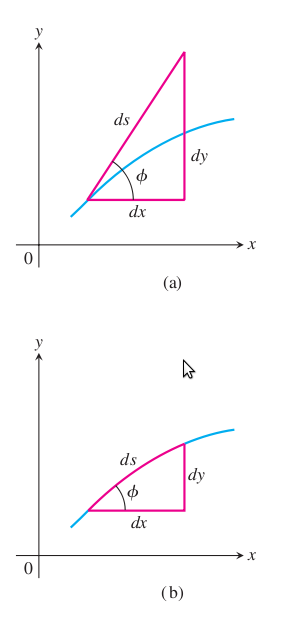
\includegraphics[height=9cm]{curve-length.png}

Egri uzunlugunun tamamini bulmak icin ise bu diferansiyel parcalari birbirine
ekleriz, yani ustteki formulun entegralini aliriz, $\int ds$ formulu entegral
sinir sartlarinin tanimlanmasi sonrasi gerekli hesabi yapacaktir.

Diyelim ki $x=0$ ve $x=1$ arasindaki hangi egrinin en kisa uzunlukta olacagini
bulmak istiyoruz. O zaman ustteki formulu $I$ haline getiririz:

\[ I(y) = \int_0^1 \sqrt{1 + (y')^2} dx \]

Bu formul Euler-Lagrange formuna sokulabilir bir formul degil mi? Iki noktayi
birlestirecek pek cok $y$ fonksiyonu olabilir, bizim aradigimiz en kisa olani ve
bunu ustteki $I$'yi duragan yapacak fonksiyonlar. Bu bir ornek tabii ki,
sezgisel olarak ta sonucu soyleyebiliriz, aradigimiz fonksiyon duz cizgi
olmali. 

Baslayalim: $F$ fonksiyonu nedir?

\[ F(x,y,y') = [1+(y')^2]^{1/2} \]

Bu fonksiyonun icinde $y$ olmadigina gore Euler-Lagrange'in $\phi$ (yani $y$)
iceren kismin atabiliriz. Kalanlar:

\[ 
\bigg[
\frac{d}{dx} \bigg( \frac{\partial F}{\partial y'} \bigg)
\bigg] = 0
 \]

Parantez icindeki kismi turevi hesaplayalim

\[ \frac{\partial F}{\partial y'} = \frac{1}{2}[1+(y')^2]^{-1/2}\ 2y = \frac{y'}{[1+(y')^2]^{1/2}} \]

Euler-Lagrange formulune koyarak iki tarafin entegralini alalim ve $dx$'ten
kurtulalim:

\[ 
\int \bigg[
\frac{d}{dx} \bigg( \frac{y'}{[1+(y')^2]^{1/2}} \bigg)
\bigg]dx = c 
 \]

\[ \frac{y'}{[1+(y')^2]^{1/2}}  = c \]

Sifirin entegrali bir sabit sayi olacaktir, bu sabite $c$ ismini verdik. Simdi
ustteki formulu $y'$ sol tarafta tek basina kalacak sekilde tekrar duzenleyelim:

\[ \frac{y'}{[1+(y')^2]^{1/2}}  = c  \]

\[ \frac{y'}{\sqrt{[1+(y')^2]}}  = c  \]

\[ \frac{y'^2}{1+(y')^2}  = c^2 \]

\[ \frac{1+(y')^2}{y'^2}  = \frac{1}{c^2} \]

\[ 1+\frac{1}{y'^2} = \frac{1}{c^2}  \]

\[ \frac{1}{y'^2} = \frac{1}{c^2} - 1 \]

\[ \frac{1}{y'^2} = \frac{1-c^2}{c^2}  \]

\[ y' = \sqrt{\frac{c^2}{1-c^2}} = a \]

Sagdaki sonuca bakarsak elimize gecen $c$'lerden olusan bir islem obegidir, ve
bu obek te dogal olarak yine bir sabit sonucunu verir, bu sabite $a$ ismini
verdik. Devam edelim, $y'$, yani turevi bir sabit olan fonksiyon, $y(x)$ suna
benzemez mi?

\[ y(x) = ax + b \]

ki sinir sartlari $y(x)=x$ (0 ve 1 degerleri icin). Bu formul bildigimiz
gibi bir duz cizginin formuludur! 

Demek ki Degisimsel Calculus kullanarak iki nokta arasindaki en kisa yolun duz
cizgi olacagini ispatlamis olduk.

Kaynaklar

Everstine, G. C., Numerical Solutions of Partial Differential Equations

Rao, S. S., The Finite Element Method in Engineering

Thomas' Calculus, 11. Baski

\end{document}